\documentclass[xcolor=pdftex,dvipsnames,table]{beamer}
%\usepackage{subfigure}
\usepackage{amsbsy}
\usepackage{tikz}
\usetikzlibrary{arrows}
\usepackage{amsmath,graphicx,dsfont,color}
\usepackage{amsfonts}
\usepackage{amssymb}
\usepackage{array}

\usepackage{subfig}

% makes the subfig package work
\makeatletter
\let\@@magyar@captionfix\relax
\makeatother

% subfigure counter resets every frame
\makeatletter
\@addtoreset{subfigure}{framenumber}
\makeatother

% First author and year
\bibliographystyle{apalike}

% This sets the list items of the bibliography to the same symbol used for citation.
\setbeamertemplate{bibliography item}{\insertbiblabel}

% This avoids extralines for different entries
\setbeamertemplate{bibliography entry title}{}
\setbeamertemplate{bibliography entry location}{}
\setbeamertemplate{bibliography entry note}{}

\DeclareMathOperator*{\argmin}{arg\,min}
\DeclareMathOperator*{\argmax}{arg\,max}
%Definitiona

\newcommand{\x}{\mathbf{x}}
\newcommand{\X}{\mathbf{X}}
\newcommand{\W}{\mathbf{W}} %Weight
\newcommand{\bais}{\mathbf{b}}%Bais
\newcommand{\act}{\texttt{g}}%Activation
\newcommand{\loss}{L}
\newcommand{\pdata}{\hat{p}_{\texttt{data}}}
\newcommand{\nsize}{N}
\newcommand{\nfeatures}{P}
\newcommand{\param}{\boldsymbol{\theta}}
\newcommand{\featmap}{\boldsymbol{\phi}}
\newcommand{\EV}{\mathbb{E}}







\usepackage{physics}

\AtBeginSection[]{
  \begin{frame}{Contents}
  \tableofcontents[currentsection, hideothersubsections]
  \end{frame}
}

\AtBeginSubsection[]{
  \begin{frame}{Contents}
  \tableofcontents[currentsection, hideothersubsections]
  \end{frame}
}

\setbeamertemplate{footline}[frame number]{}
\setbeamertemplate{navigation symbols}{}
\setbeamertemplate{section in toc}[square]
\setbeamertemplate{items}[square]

\title{Artificial neural networks and backpropagation}
\author{E. Decencière}
\date{MINES ParisTech\\
  PSL Research University\\
  Center for Mathematical Morphology
}
\titlegraphic{
\includegraphics[height=1.7cm]{../graphics/logoemp}}

\useinnertheme{rounded}
\usecolortheme{rose}

%%%%%%%%%%%%%%%%%%%%%%%%%%%%%%%%%%%%%%%%%%%%%%%%%%
%%%%%%%%%%%%%%%%%%%%%%%%%%%%%%%%%%%%%%%%%%%%%%%%%%
\begin{document}
\begin{frame}
\titlepage
\end{frame}

\frame{
\frametitle{Contents}
\tableofcontents[hidesubsections]
}


%%%%%%%%%%%%%%%%%%%%%%%%%%%%%%%%%%%%%%%%%%%%%%%%%%
\section{Introduction}
%%%%%%%%%%%%%%%%%%%%%%%%%%%%%%%%%%%%%%%%%%%%%%%%%%

\frame{
\frametitle{Artificial neural networks and deep learning history}


\begin{block}{}
  For a very complete state of the art on deep learning, see the overview by Schmidhuber \cite{schmidhuber_deep_2015}.
\end{block}

\begin{itemize}
\item 1958: Rosenblatt's perceptron \cite{rosenblatt_perceptron:_1958}
\item 1980's: the backpropagation algorithm (see, for example, the work of Le Cun \cite{lecun_procedure_1985})
\item 2006-: CNN implementations using Graphical Processing Units (GPU): up to a 50 speed-up factor.
\item 2011-: super-human performances \cite{ciresan_committee_2011}
\item 2012: Imagenet image classification won by a CNN \cite{krizhevsky_imagenet_2012}.

\end{itemize}

}

%%%%%%%%%%%%%%%%%%%%%%%%%%%%%%%%%%%%%%%%%%%%%%%%%%
\section{Artificial neuron}
%%%%%%%%%%%%%%%%%%%%%%%%%%%%%%%%%%%%%%%%%%%%%%%%%%

\frame{
\frametitle{Neuron}

\begin{figure}
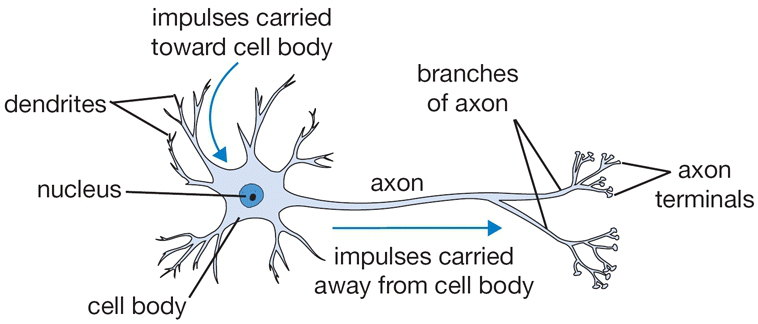
\includegraphics[height=3cm]{../graphics/neuron}
\end{figure}

\begin{itemize}
\item The human brain contains 100 billion ($10^{11}$) neurons
\item A human neuron can have several thousand dendrites
\end{itemize}

}

%%%%%%%%%%%%%%%%%%%%%%%%%%%%%%%%%%%%%%%%%%%%%%%%%%

\frame{
\frametitle{Artificial neuron}

\begin{figure}
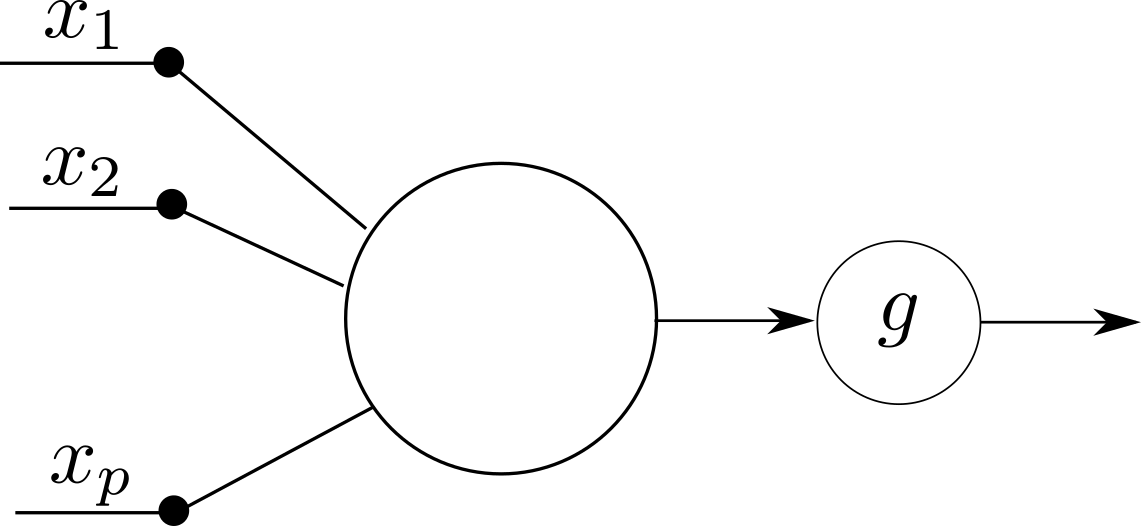
\includegraphics[height=3cm]{../graphics/neurone_general}
\end{figure}

\begin{block}{General principle}
An artificial neuron takes $p$ inputs $\{x_i\}_{1 \leq i \leq p}$, combines them to obtain a single value, and applies an \alert{activation function} to the result.
\end{block}

\begin{itemize}
\item The first artificial neuron model was proposed by \cite{mcculloch_logical_1943}
\item Input and output signals were binary
\item Input dendrites could be inhibitory or excitatory
\end{itemize}

}

%%%%%%%%%%%%%%%%%%%%%%%%%%%%%%%%%%%%%%%%%%%%%%%%%%

\frame{
\frametitle{Artificial neuron}

\begin{figure}
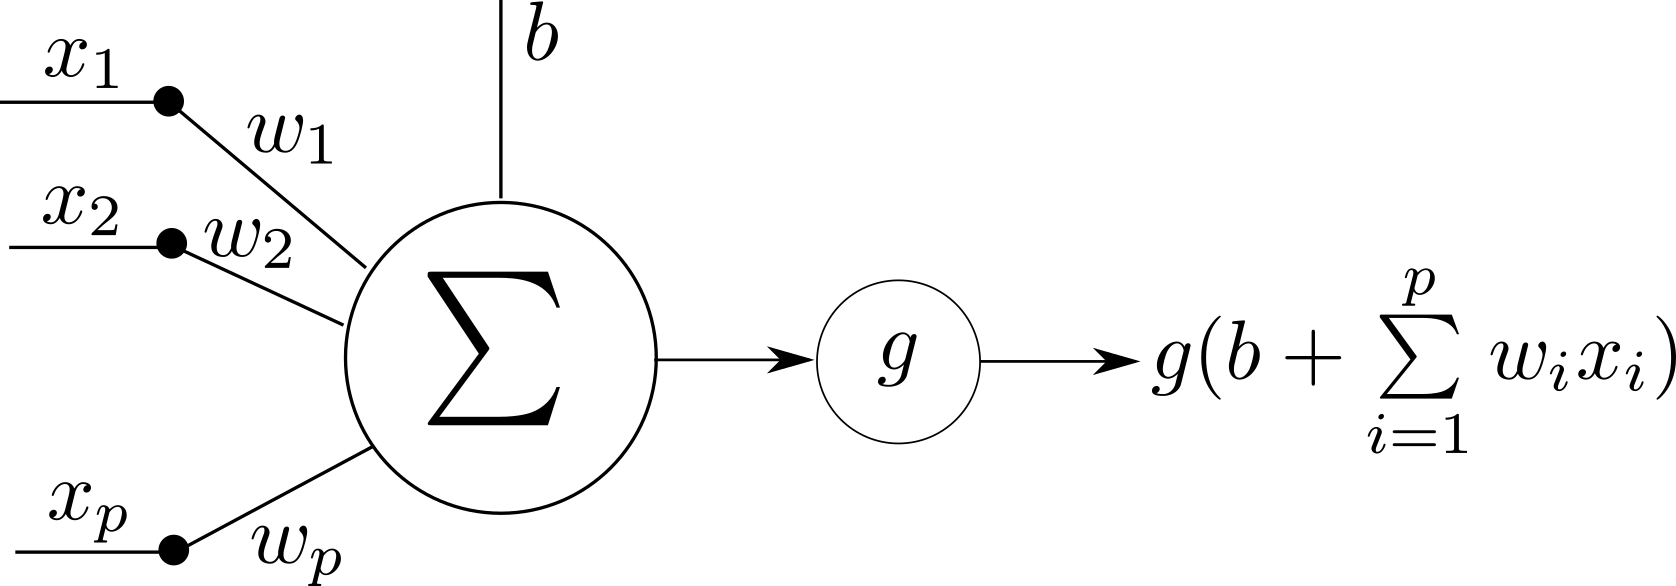
\includegraphics[height=3cm]{../graphics/neurone}
\end{figure}

\begin{block}{Classical neuron}
  \alert{Bias} $\bias$ is a variable linked to the neuron. The \alert{activation function} $\act$ somehow decides, depending on the input, if a signal (the neuron's \alert{activation}) is produced.
\end{block}

}

%%%%%%%%%%%%%%%%%%%%%%%%%%%%%%%%%%%%%%%%%%%%%%%%%%

\frame{
  \frametitle{Activation: binary}

  \begin{columns}
    \begin{column}{.5\textwidth}
      \[
      g(x)=
      \begin{cases}
        1,& \text{if } x > 0\\
        0,              & \text{otherwise}
      \end{cases}
      \]

    \end{column}

    \begin{column}{.5\textwidth}
      \begin{figure}
        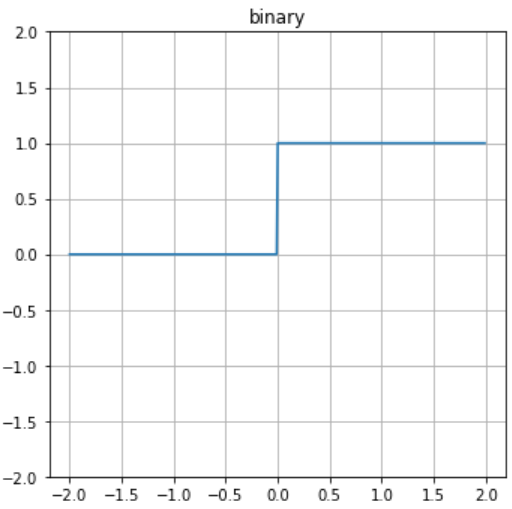
\includegraphics[width=.8\textwidth]{../graphics/act_bin.png}
      \end{figure}


    \end{column}
  \end{columns}

  \begin{block}{Remarks}
    \begin{itemize}
    \item Biologically inspired
    \item[+] Simple to compute
    \item[+] High abstraction
    \item[-] Gradient nil except on one point
    \end{itemize}
  \end{block}


}

%%%%%%%%%%%%%%%%%%%%%%%%%%%%%%%%%%%%%%%%%%%%%%%%%%

\frame{
  \frametitle{Activation: sigmoid}

  \begin{columns}
    \begin{column}{.5\textwidth}
      \[
      g(x)= \frac{1}{1 + e^{-x}}
      \]
    \end{column}

    \begin{column}{.5\textwidth}
      \begin{figure}
        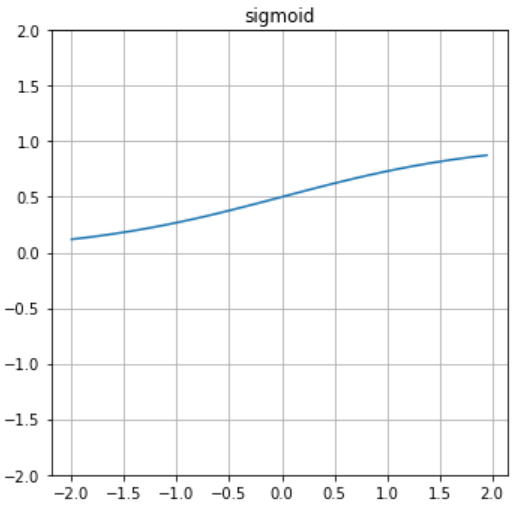
\includegraphics[width=.8\textwidth]{../graphics/act_sigm.png}
      \end{figure}


    \end{column}
  \end{columns}

  \begin{block}{Remarks}
    \begin{itemize}
    \item[+] Similar to binary activation, but with usable gradient
    \item[-] However, gradient tends to zero when input is far from zero
    \item[-] More computationally intensive
    \end{itemize}
  \end{block}



}

%%%%%%%%%%%%%%%%%%%%%%%%%%%%%%%%%%%%%%%%%%%%%%%%%%

\frame{
  \frametitle{Activation: hyperbolic tangent}

  \begin{columns}
    \begin{column}{.5\textwidth}
      \[
      g(x)= \frac{e^x - e^{-x}}{e^x + e^{-x}}
      \]
    \end{column}

    \begin{column}{.5\textwidth}
      \begin{figure}
        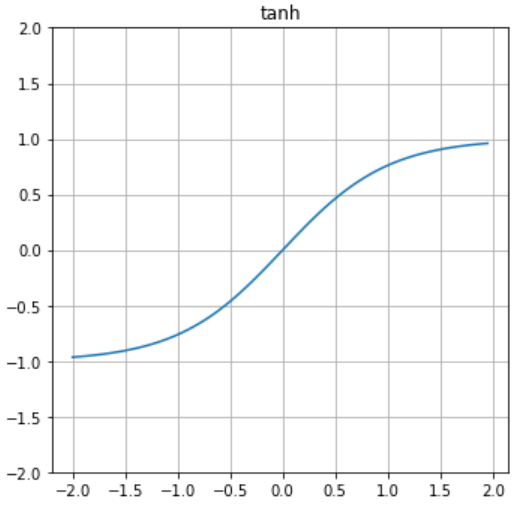
\includegraphics[width=.8\textwidth]{../graphics/act_tanh.png}
      \end{figure}


    \end{column}
  \end{columns}

  \begin{block}{Remarks}
    \begin{itemize}
    \item Similar to sigmoid
    \end{itemize}
  \end{block}



}


%%%%%%%%%%%%%%%%%%%%%%%%%%%%%%%%%%%%%%%%%%%%%%%%%%

\frame{
  \frametitle{Activation: rectified linear unit}

  \begin{columns}
    \begin{column}{.5\textwidth}
      \[
      g(x)=
      \begin{cases}
        x,& \text{if } x > 0\\
        0,              & \text{otherwise}
      \end{cases}
      \]
    \end{column}

    \begin{column}{.5\textwidth}
      \begin{figure}
        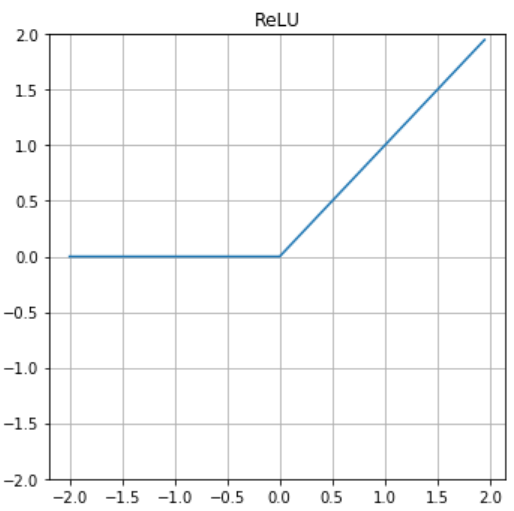
\includegraphics[width=.8\textwidth]{../graphics/act_relu.png}
      \end{figure}


    \end{column}
  \end{columns}

  \begin{block}{Remarks}
    \begin{itemize}
    \item[+] Usable gradient when activated
    \item[+] Fast to compute
    \item[+] High abstraction
    \end{itemize}
  \end{block}



}

%%%%%%%%%%%%%%%%%%%%%%%%%%%%%%%%%%%%%%%%%%%%%%%%%%

\frame{
\frametitle{What can an artifical neuron compute?}

\begin{figure}
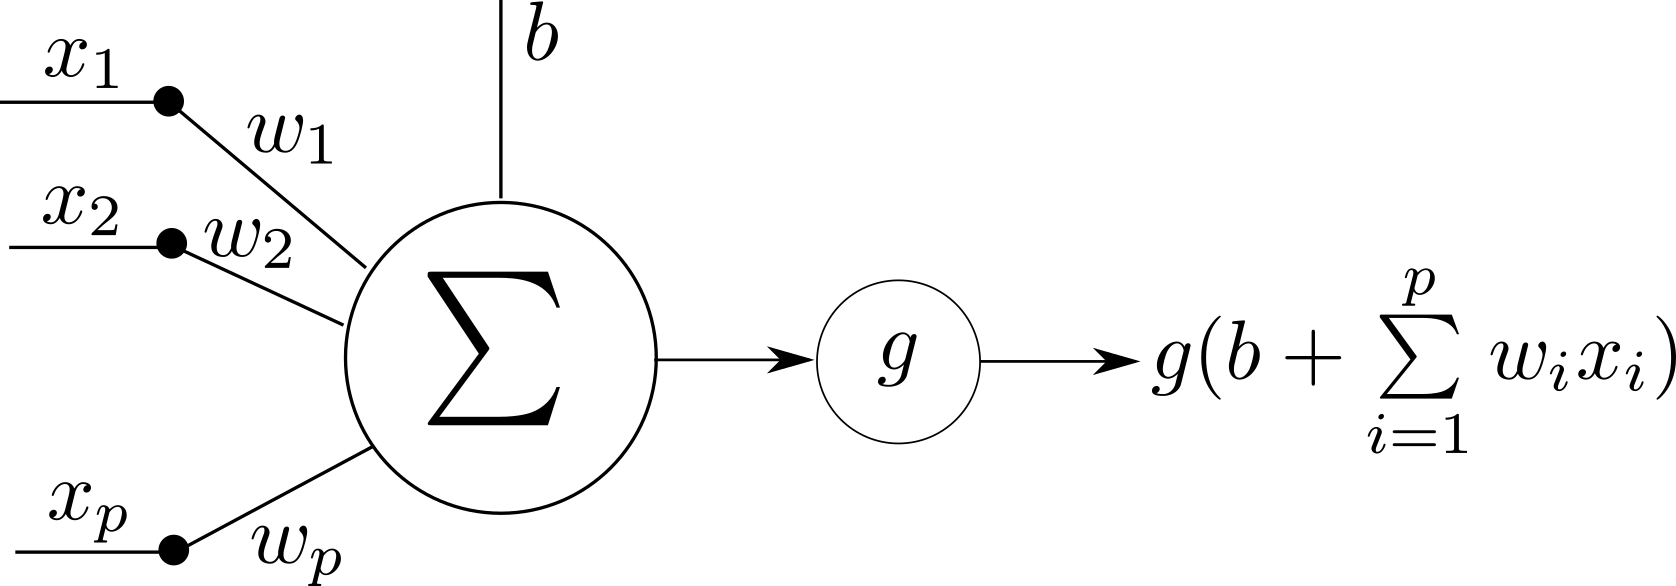
\includegraphics[height=3cm]{../graphics/neurone}
\end{figure}

\begin{block}{}
  In $\R^p$ ,
  $b + \sum\limits_{i=0}^p w_ix_i = 0$
  gives a hyperplane. For a given point
  $\x = \{x_0, \ldots, x_p\}$,
  decisions are made according to the side of the hyperplane it belongs to.
\end{block}

}

%%%%%%%%%%%%%%%%%%%%%%%%%%%%%%%%%%%%%%%%%%%%%%%%%%

\frame{
\frametitle{The power of an artificial neuron: illustration}

\begin{figure}
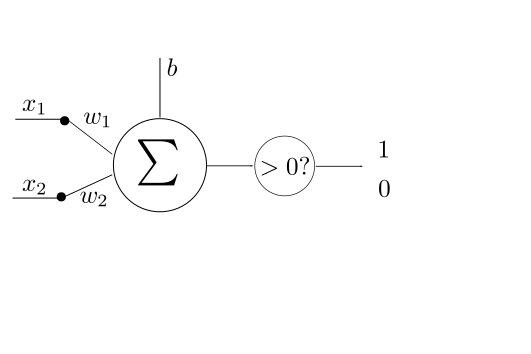
\includegraphics[height=3cm]{../graphics/neurone_simple}
\end{figure}



}

%%%%%%%%%%%%%%%%%%%%%%%%%%%%%%%%%%%%%%%%%%%%%%%%%%

\frame{
\frametitle{Neural network}


\begin{figure}
  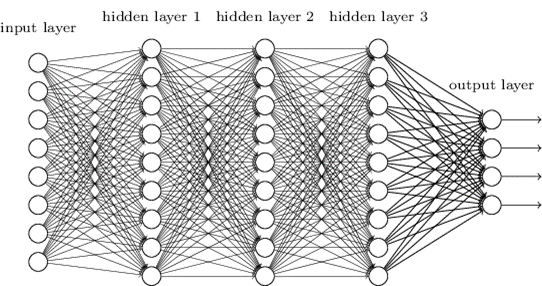
\includegraphics[height=5cm]{../graphics/network.png}
\end{figure}

{\small(from http://www.jtoy.net)}

}


%%%%%%%%%%%%%%%%%%%%%%%%%%%%%%%%%%%%%%%%%%%%%%%%%%

\frame{
\frametitle{Convolutional neural networks (ConvNets or CNNs)}

\begin{figure}
  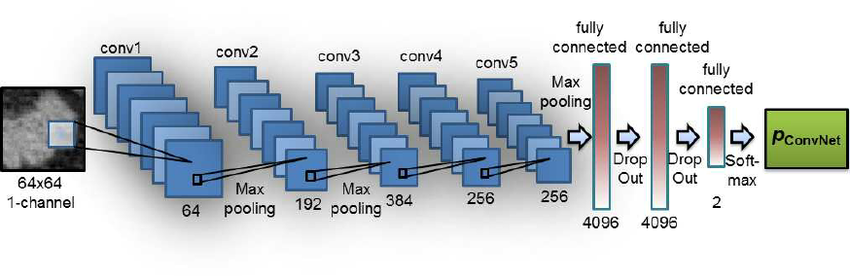
\includegraphics[height=3cm]{../graphics/convnet.png}
\end{figure}


(from https://www.researchgate.net)


}

%%%%%%%%%%%%%%%%%%%%%%%%%%%%%%%%%%%%%%%%%%%%%%%%%%

\frame{
\frametitle{The triggering factor to the success of neural networks}

\begin{itemize}

\item Appropriate architectures: graphical processing units (GPUs)
\item Optimized software
\item Large annotated databases

\end{itemize}

}

%%%%%%%%%%%%%%%%%%%%%%%%%%%%%%%%%%%%%%%%%%%%%%%%%
%%%%%%%%%%%%%%%%%%%%%%%%%%%%%%%%%%%%%%%%%%%%%%%%%
\section{Deep learning today and tomorrow}


%%%%%%%%%%%%%%%%%%%%%%%%%%%%%%%%%%%%%%%%%%%%%%%%%%

\frame{
\frametitle{Practical considerations}

For a deep-learning solution to work, you need:

\begin{itemize}

\item A lot of annotated data
\item A lot of fiddling (different architectures; hyper-parameters)
\item GPUs, at least from training

\end{itemize}

Deep learning can produce astonishing results \cite{nguyen_deep_2015}...
\begin{figure}
  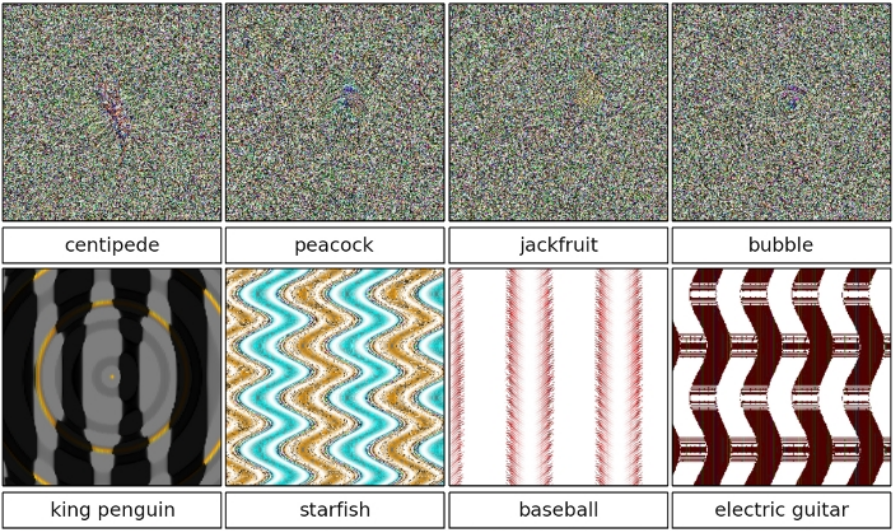
\includegraphics[height=3cm]{../graphics/dl_easily_fooled.png}
\end{figure}


}


%%%%%%%%%%%%%%%%%%%%%%%%%%%%%%%%%%%%%%%%%%%%%%%%%%

\frame{
\frametitle{The web giants}

\begin{itemize}

\item Google, Facebook, Microsoft, Amazon etc. are actively investing in deep-learning
  \item Competition is intense
  \item Most of them are sharing their deep learning libraries

\end{itemize}

}




%%%%%%%%%%%%%
\begin{frame}{Backpropagation through a fully connected layer}
\begin{figure}
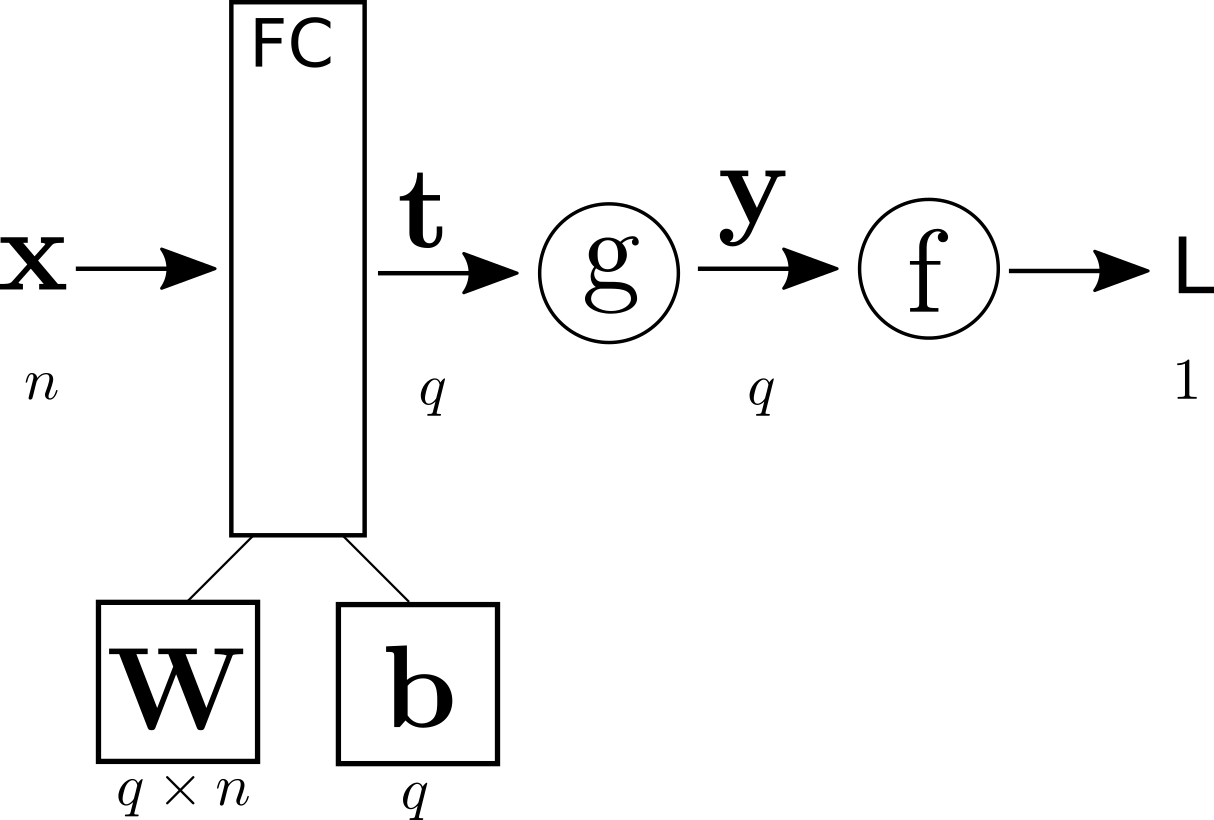
\includegraphics[width=0.5\textwidth]{../graphics/bp_fc.png}
\end{figure}

Setup:
\begin{eqnarray*}
n, q \in \N^*\\
\x \in \R^n \\
\W \in \R^q \times \R^n \\
\bias, \mathbf{t}, \y \in \R^q \\
\loss \in \R
\end{eqnarray*}

\end{frame}

%%%%%%%%%%%%%
\begin{frame}{Backpropagation through a fully connected layer}
\begin{figure}
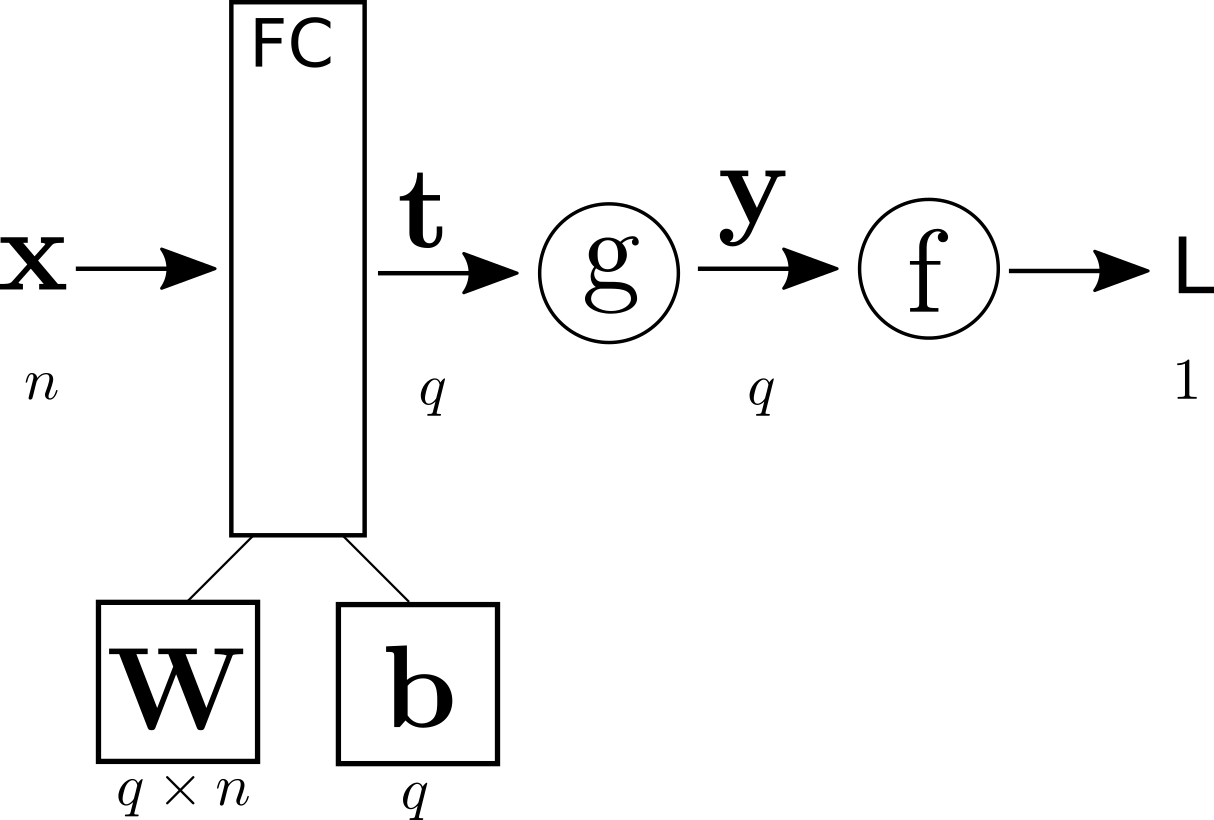
\includegraphics[width=0.5\textwidth]{../graphics/bp_fc.png}
\end{figure}

\begin{columns}
  \begin{column}{0.5\textwidth}
    Forward pass:
    \begin{eqnarray*}
      \mathbf{t} &=& \W\x + \bias \\
      \y &=& \act(\W\x + \bias) \\
      \loss &=& \loss(\y)
    \end{eqnarray*}
  \end{column}

  \begin{column}{0.5\textwidth}
    Local gradients:
    \begin{eqnarray*}
      \pdv{\mathbf{t}}{\W} &=& \x^t \\
      \pdv{\mathbf{t}}{\bias} &=& 1 \\
      \pdv{\y}{\mathbf{t}} &=& \act'
    \end{eqnarray*}
  \end{column}
\end{columns}

\end{frame}

%%%%%%%%%%%%%
\begin{frame}{Backpropagation through a fully connected layer}
  \begin{figure}
    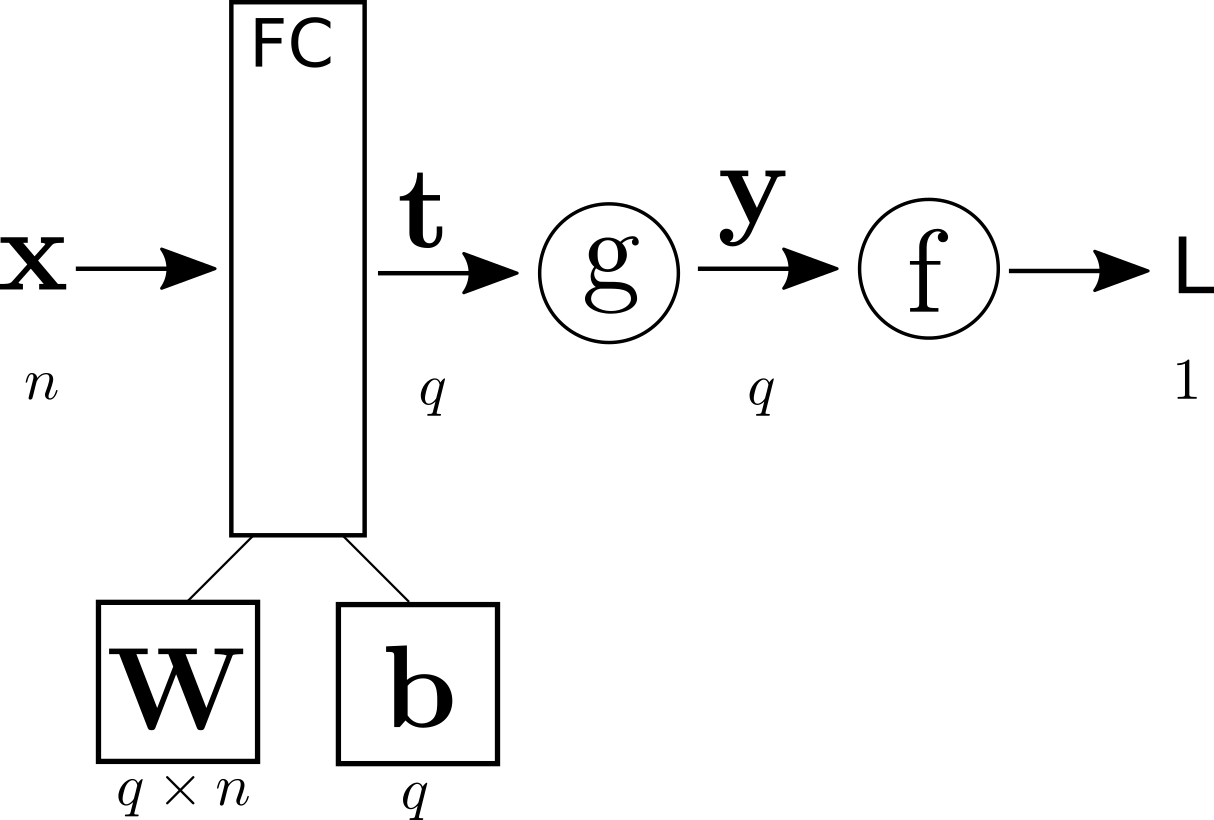
\includegraphics[width=0.5\textwidth]{../graphics/bp_fc.png}
  \end{figure}

  Backpropagation:
  \begin{eqnarray*}
    \pdv{\loss}{\mathbf{t}} &=& \pdv{\loss}{\y}.\pdv{\y}{\mathbf{t}} \\
                           &=& \pdv{\loss}{\y} \odot \act'(\mathbf{t}) \\
  \end{eqnarray*}

\end{frame}

%%%%%%%%%%%%%
\begin{frame}{Backpropagation through a fully connected layer}
  \begin{figure}
    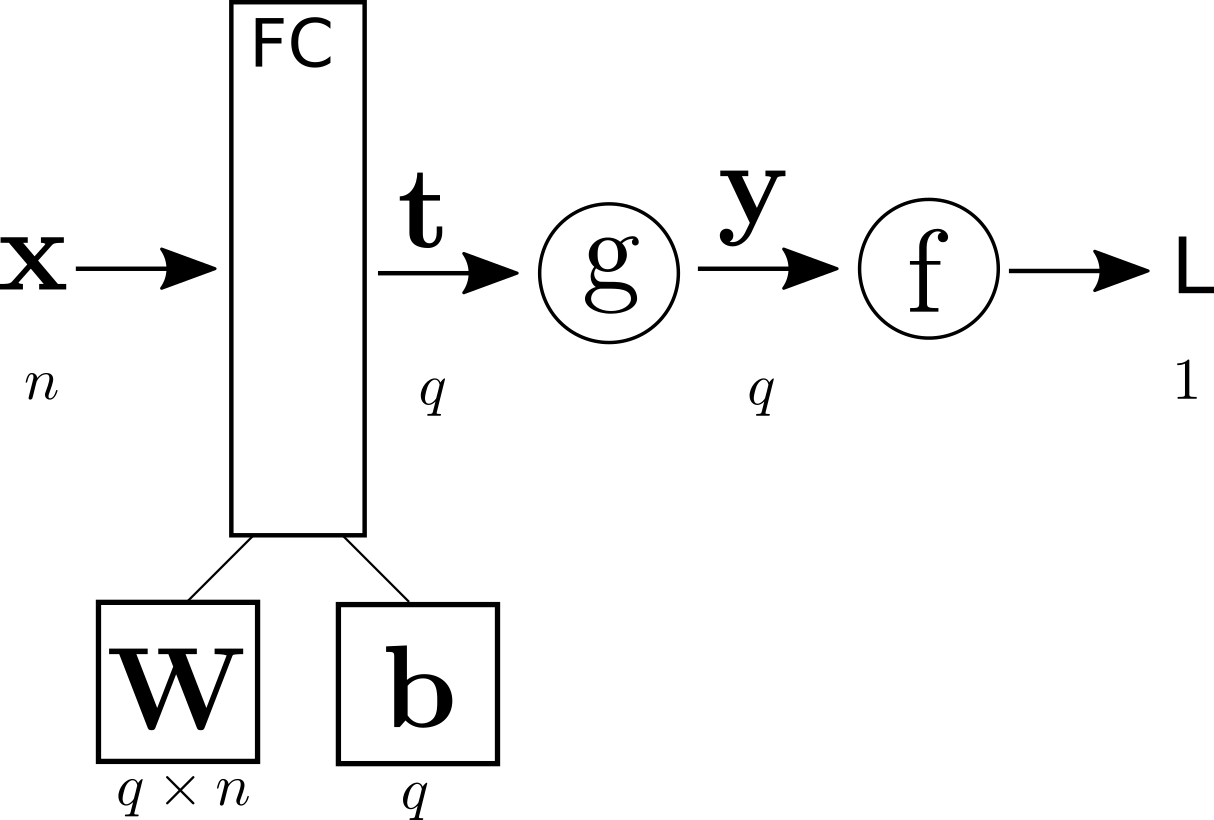
\includegraphics[width=0.5\textwidth]{../graphics/bp_fc.png}
  \end{figure}

  Backpropagation:
  \begin{columns}
    \begin{column}{.5\textwidth}
      \begin{eqnarray*}
        \pdv{\loss}{\W} &=& \pdv{\loss}{\mathbf{t}}.\pdv{\mathbf{t}}{\W} \\
                   &=& \pdv{\loss}{\y} \odot \act'(\mathbf{t}).\x^t
      \end{eqnarray*}
    \end{column}

  \begin{column}{.5\textwidth}
  \begin{eqnarray*}
    \pdv{\loss}{\bias} &=&  \pdv{\loss}{\y} \odot \act'(\mathbf{t})
  \end{eqnarray*}
  \end{column}
\end{columns}


\end{frame}

%%%%%%%%%%%%%%%%%%%%%%%%%%%%%%%%%%%%%%%%%%%%%%%%%%
\section*{References}

%%%%%%%%%%%%%%%%%%%%%%%%%%%%%%%%%%%%%%%%%%%%%%%%%%

\frame[allowframebreaks]{

\scriptsize

\frametitle{References}

%\bibliographystyle{amsalpha}
%\bibliographystyle{apalike}

\bibliography{edf.bib}

\normalsize

}

%%%%%%%%%%%%%%%%%%%%%%%%%%%%%%%%%%%%%%%%%%%%%%%%%%
%%%%%%%%%%%%%%%%%%%%%%%%%%%%%%%%%%%%%%%%%%%%%%%%%%
%%%%%%%%%%%%%%%%%%%%%%%%%%%%%%%%%%%%%%%%%%%%%%%%%%

\end{document}
